\section{Auswertung}
\label{sec:Auswertung}
\subsection{Vermessung von Spektrallinien}
\label{subsec:a0}
Es besteht die Möglichkeit allein durch Abzählen der Kanäle und der entsprechenden Zählergebnisse die Höhe, die Lage und den Inhalt einer Spektrallinie anzugeben.
Die Ergebnisse dieser Methode können jedoch nicht immer eindeutig angegeben werden, sodass eine unabhängige Auswertung unmöglich wird.
Hier wird daher eine andere Methode gewählt.
Zunächst wird die Lage einer Spektrallinie, wie oben auch, auf den Kanal mit dem höchsten Zählergebnis in einer hinreichend großen Umgebung geschätzt.
Um den so abgelesenen Kanal herum wird über die jeweils 20 oberhalb und unterhalb liegenden Kanäle eine Gauß-Funktion
\begin{align}
g(k)=c_1\exp\left(-c_2(k-c_3)^2\right)+c_4
\end{align}
an die Messdaten gefittet.
Dabei entspricht $c_1$ der Höhe der Spektrallinie und $c_3$ ihrer Lage.
Hier ist sofort ein Vorteil dieser Methode zu erkennen, denn die Lage einer Spektrallinie kann nun präziser als die Auflösung der Kanalskala angegeben werden.
Die Formel
\begin{align}
  \label{eqn:inhalt}
  \int_\infty^\infty c_1\exp\left(-c_2(k-c_3)^2\right) dk = c_1 \sqrt{\frac{\pi}{c_2}}
\end{align}
zeigt, dass $c_1$ und $c_2$ zusammen ein Maß für den Inhalt einer Spektrallinie sind.
Der Parameter $c_4$ dient dazu Störeffekte wie das Compton-Kontinuum oder die Untergrundstrahlung aus den folgenden Rechnungen zu eliminieren.
Er wird deshalb im Folgenden nicht weiter berücksichtigt.
Diese und jede weitere Regressionsrechnung in dieser Auswertung wird mithilfe der Funktion \textit{curve\_ fit} aus dem Python Paket \textit{scipy.optimize} durchgeführt.
Fehlerrechnungen werden ebenfalls von Python übernommen.
Dazu wird das Paket \textit{uncertainties} verwendet.
\FloatBarrier
\subsection{Kalibrierung und Bestimmung der Effizienz}
\label{subsec:a1}
Um das Energiespektrum für unbekannte Strahler sinnvoll interpretieren zu können,
ist eine Kalibrierung der Energieskala notwendig. Dazu wird das linienreiche Spektrum eines Europium-152 Strahlers betrachtet, welches in Abbildung \ref{fig:spektrum_eu} dargestellt ist.
\begin{figure}
 \centering
 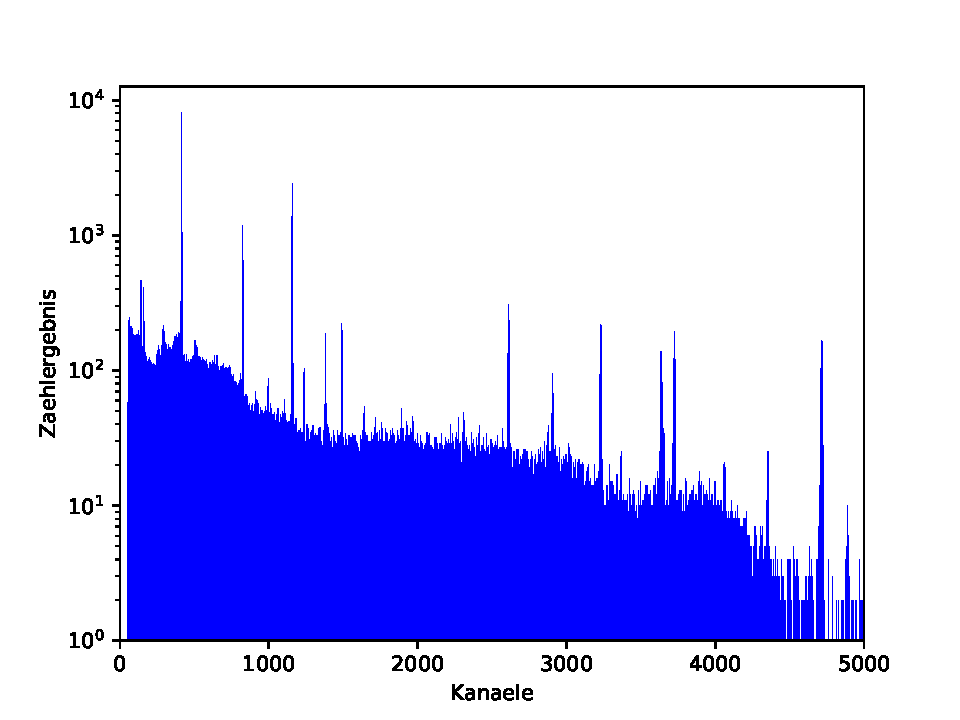
\includegraphics[width=0.8\textwidth]{python/plots/spec1.pdf}
 \caption{Rohdaten der Vermessung des Europium-152 Spektrums.}
 \label{fig:spektrum_eu}
 \end{figure}
Die in Tabelle \ref{tab:atab1} angegebenen Kanäle der Spektrallinien werden nach dem in Abschnitt \ref{subsec:a0} beschriebenen Verfahren bestimmt.
\begin{table}
\centering
\caption{Gemessene Kanäle $k$, zugehörige Energieliteraturwerte $E_{\text{lit}}$ und durch die Kalibrierung aus den Kanälen bestimmten Energien $E_{\gamma}$ eines Europium-152 Gammaspektrums, sowie Literaturwerte für die Emissionswahrscheinlichkeit $W$ der Spektrallinien, die nach Kap.~\ref{subsec:a0} berechneten Inhalte $I$ der Peaks und die daraus berechnete Effizienz $Q$ \cite{sample}.}
\begin{tabular}{c c c c c c}
\hline \\
$k$ &$E_{\gamma}$ / keV & $E_{\text{lit}}$ / keV &  $W$ / \% & $I$ & $Q$ / \% \\
\hline \\
414,10 $\pm$ 0,01 & 121,97 $\pm$ 0,01 & 121,78 & 28,60 & 28310$\pm$90 & 45,5$\pm$0,6 \\
825,73 $\pm$ 0,02 & 244,97 $\pm$ 0,01 & 244,70 & 7,60 & 4770$\pm$40 & 28,80$\pm$0,5 \\
996,99 $\pm$ 0,23 & 296,15 $\pm$ 0,07 & 295,94 & 0,40 & 230$\pm$30 & 27,0$\pm$3,0 \\
1158,61 $\pm$ 0,01 & 344,44 $\pm$ 0,01 & 344,30 & 26,50 & 11700$\pm$70 & 20,3$\pm$0,3 \\
1381,69 $\pm$ 0,06 & 411,10 $\pm$ 0,02 & 411,12 & 2,20 & 740$\pm$20 & 15,4$\pm$0,5 \\
1492,22 $\pm$ 0,05 & 444,13 $\pm$ 0,01 & 443,96 & 3,10 & 1010$\pm$20 & 15,0$\pm$0,4 \\
2275,02 $\pm$ 0,82 & 678,05 $\pm$ 0,25 & 678,00 & 2,00 & 40$\pm$10 & 1,00$\pm$0,3 \\
2310,57 $\pm$ 0.33 & 688,67 $\pm$ 0,10 & 688,67 & 0,90 & 240$\pm$20 & 12,0$\pm$1,0 \\
2611,88 $\pm$ 0,06 & 778,71 $\pm$ 0,02 & 778,90 & 12,90 & 2320$\pm$40 & 8,3$\pm$0,2 \\
2907,84 $\pm$ 0,18 & 867,15 $\pm$ 0,05 & 867,37 & 4,20 & 640$\pm$30 & 7,0$\pm$0,3 \\
3232,04 $\pm$ 0,09 & 964,02 $\pm$ 0,03 & 964,08 & 14,60 & 2080$\pm$40 & 6,6$\pm$0,2 \\
3368,48 $\pm$ 0,47 & 1004,79 $\pm$ 0,14 & 1005,30 & 0,60 & 90$\pm$10 & 7,0$\pm$1,0 \\
3638,77 $\pm$ 0,15 & 1085,56 $\pm$ 0,04 & 1085,90 & 10,20 & 1170$\pm$40 & 5,3$\pm$0,2 \\
3726,06 $\pm$ 0,10 & 1111,65 $\pm$ 0,03 & 1112,10 & 13,60 & 1830$\pm$40 & 6,2$\pm$0,2 \\
4353,18 $\pm$ 0,38 & 1299,04 $\pm$ 0,11 & 1299,10 & 1,60 & 160$\pm$20 & 4,6$\pm$0,5 \\
4716,47 $\pm$ 0,16 & 1407,60 $\pm$ 0,05 & 1408,00 & 21,00 & 2290$\pm$70 & 5,0$\pm$0,2 \\
4890,43 $\pm$ 0,59 & 1459,58 $\pm$ 0,18 & 1457,60 & 0,50 & 180$\pm$50 & 16,0$\pm$5,0\\
\hline
\end{tabular}
\label{tab:atab1}
\end{table}
In Abbildung \ref{fig:Kalibrierung} werden die entsprechenden Kanäle gegen die Literaturwerte des Europium-152 Spektrums aufgetragen.
Über eine lineare Ausgleichsrechnung wird die Kalibrationsfunktion
\begin{align*}
E(k) &= s \cdot k + b \text{, mit}\\
  s &= \SI{0.29882+-0.00009}{\kilo\electronvolt}\\
  b &= \SI{ -1.8+-0.3}{\kilo\electronvolt}
\end{align*}
zwischen Kanalnummern und Energien in keV bestimmt.
\begin{figure}
\centering
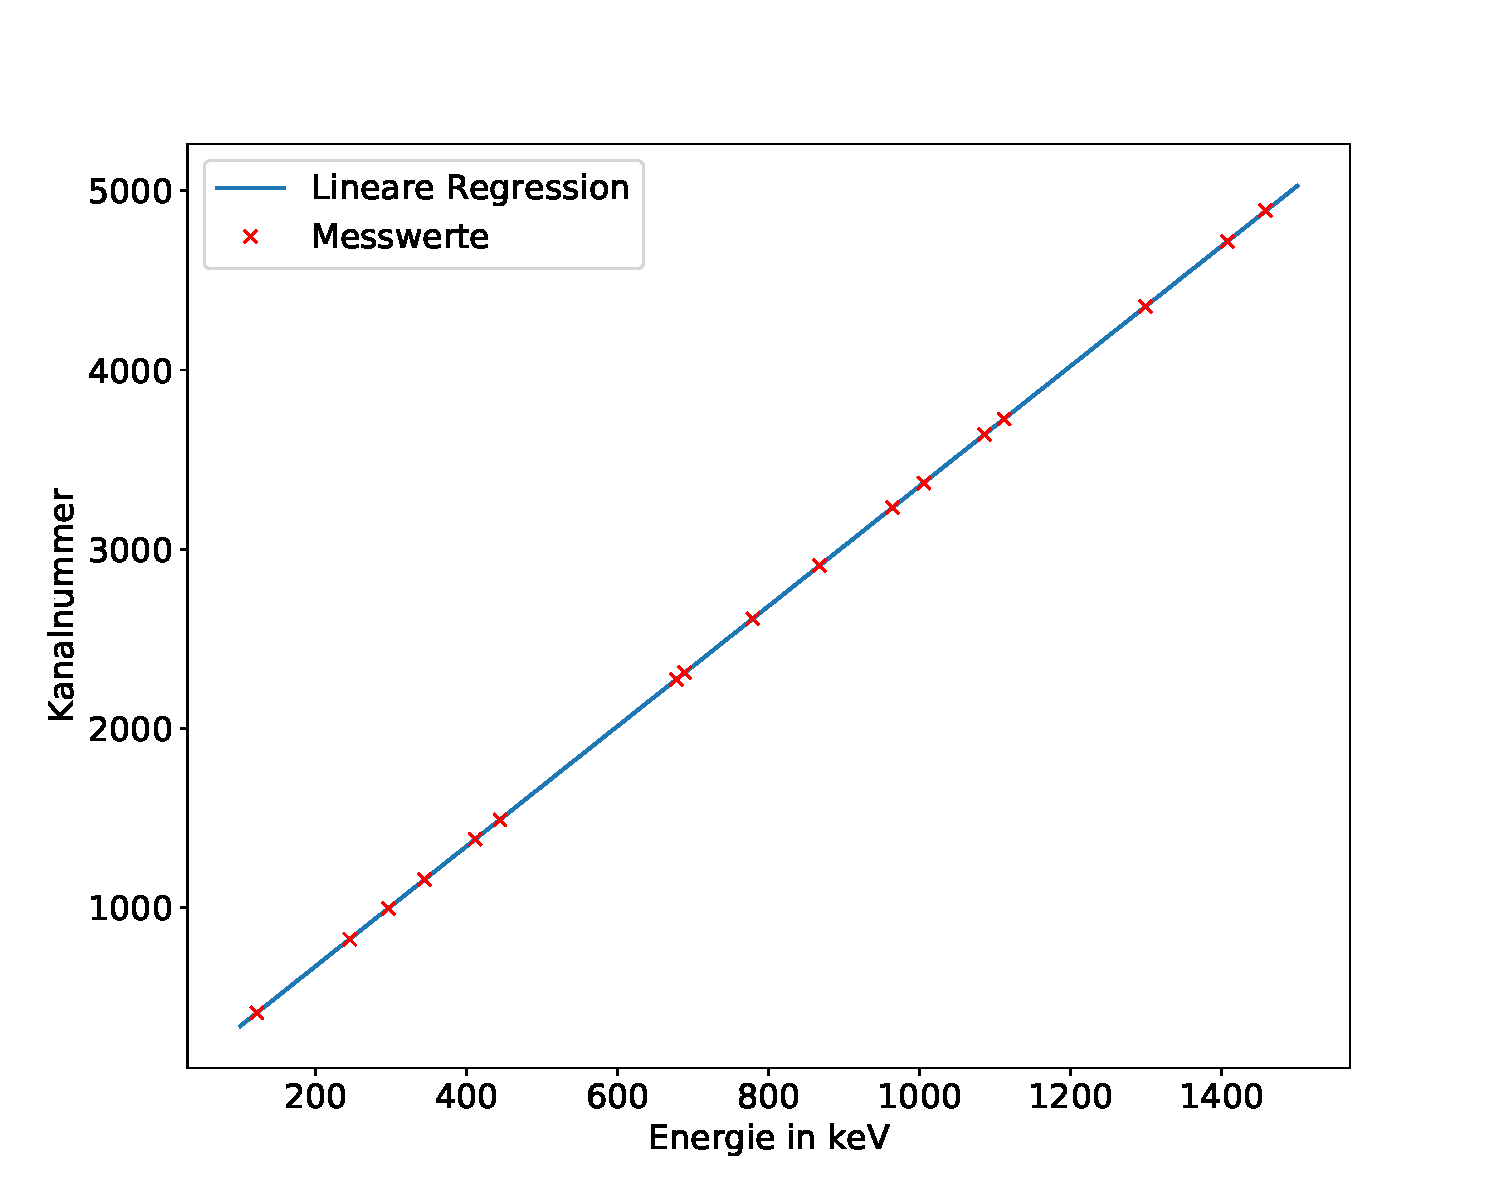
\includegraphics[width=0.8\textwidth]{python/plots/kalibrierung.pdf}
\caption{Lineare Regression der Messwerte aus Tabelle \ref{tab:atab1} für Europium-152.}
\label{fig:Kalibrierung}
\end{figure}
Mit Gleichung \eqref{eqn:effizienz} soll die Effizienz des Detektors bestimmt werden.
Um die dazu nötige Aktivität des Europium-152 zum Zeitpunkt der Messung zu bestimmen, wird das exponentielle Zerfallsgesetz
\begin{align}
A_\text{Messung}=A_0\exp\left(\frac{\log(2)}{T_{\frac{1}{2}}}\Delta t\right)
\end{align}
verwendet.
Die Aktivität $A_0$ am 01.10.2000 betrug $\SI{4130+-60}{\becquerel}$ und die Halbwertszeit von Europium-152 beträgt $\SI{4943+-5}{\day}$ \cite{sample}.
Die Anzahl der Tage zwischen dem 01.10.2000 und dem Tag der Durchführung beträgt $\Delta t=\SI{6084}{\day}$.
Daraus ergibt sich eine Aktivität von
\begin{align*}
A_\text{Messung}=\SI{1760+-26}{\becquerel} \text{ .}
\end{align*}
Leider wurde der Abstand $d$ zwischen der Probe und der Schutzhaube des Detektors nicht gemessen.
Der Wert von $d=\SI{8.8}{\centi\meter}$ wird deshalb dem Protokoll einer befreundeten Gruppe entnommen \cite{abstand}.
Der Radius des Detektors beträgt $r=\SI{2.25}{\centi\meter}$ \cite{sample}.
Aus
\begin{align}
\Omega=2\pi\left( 1- \frac{a}{\sqrt{a^2+r^2}}\right)
\end{align}
lässt sich dann der Raumwinkel $\Omega=\SI{0.177}{}$ berechnen, wobei $a=\SI{8.8}{\centi\meter}+\SI{1.5}{\centi\meter}=\SI{10.3}{\centi\meter}$ gewählt wird, da der wahrscheinlichste Absorptionspunkt ca. $\SI{1.5}{\centi\meter}$ unter der Schutzhaube liegt \cite{sample}.
Mit diesem Wert und den aus den Gauß-Fits berechneten Flächeninhalten der Gauß-Funktionen lassen sich nun die in Tabelle \ref{tab:atab1} angegebenen Effizienzen berechnen.
Dabei ist zu Berücksichtigen, dass die Zählrate aus Formel \ref{eqn:effizienz} gerade den Inhalten geteilt durch die Messdauer $t_\text{Messung}=\SI{7764}{\second}$ entspricht.
Es wird angenommen, dass die Effizienz $Q$ mit steigender Energie wie eine Potenzfunktion
\begin{align}
Q(E)=c E^{d}
\end{align}
abnimmt.
Die in Abbildung \ref{fig:Effizienz} dargestellte Regressionsrechnung liefert die Parameter
\begin{align*}
c&=\SI{150+-100}{\per\kilo\electronvolt}\\
d&=\SI{-1.10+-0.1}{}\text{ .}
\end{align*}
\begin{figure}
\centering
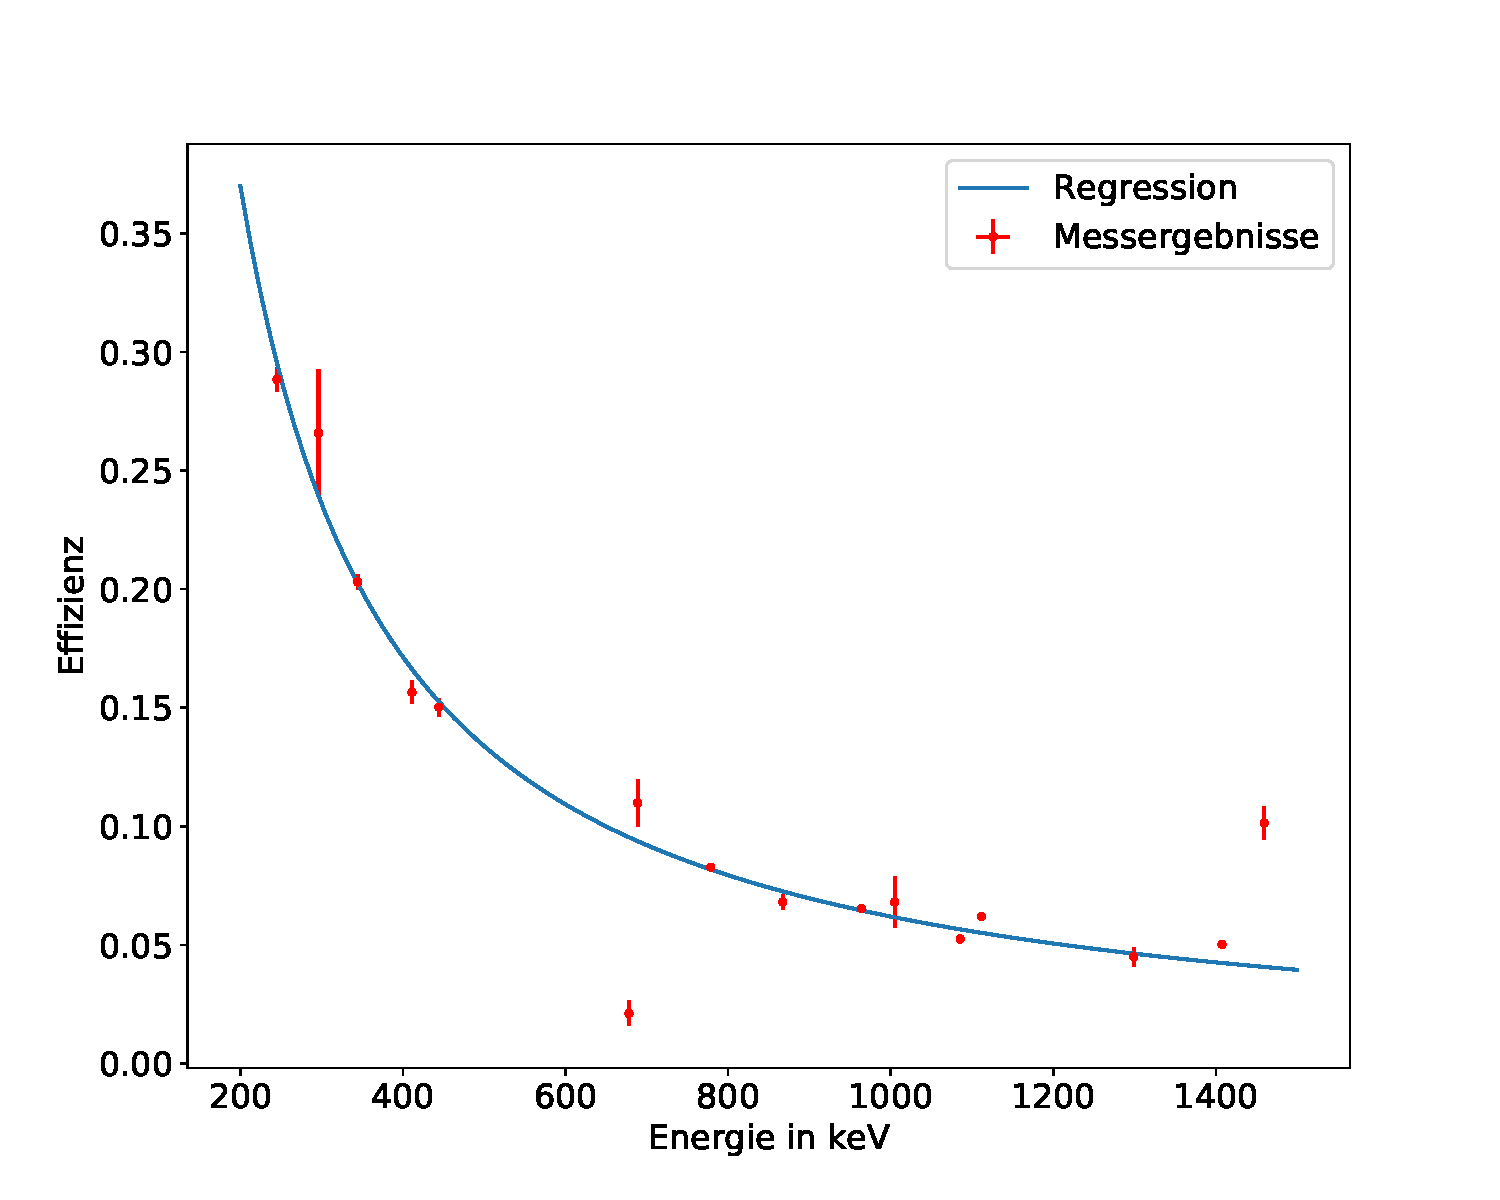
\includegraphics[width=0.8\textwidth]{python/plots/effizienz.pdf}
\caption{Darstellung der Abnahme der Effizienz mit Steigender Energie durch eine Regressionsrechnung. Energien unterhalb von $\SI{150}{\electronvolt}$ werden nicht betrachtet.}
\label{fig:Effizienz}
\end{figure}

\FloatBarrier

\subsection{Bestimmungen von Detektoreigenschaften}
\label{subsec:a2}
Um Informationen über Detektoreigenschaften, wie die Energieauflösung, zu gewinnen, wird das Spektrum eines Caesium-137 Strahlers untersucht.
Die Messzeit beträgt $\SI{3028}{\second}$ Eine graphische Darstellung des aufgenommenen
Spektrums, ist in Abbildung \ref{fig:spectrum_caesium} gegeben. Um die Energieskala zu erhalten,
wird die in Abschnitt \ref{subsec:a1} gefundene Kalibrierungsfunktion angewendet.

\subsubsection{Vermessung des Photopeaks}
\label{subsubsec:a21}
Zunächst wird die Position des Phototpeaks, mithilfe eines wie in Abschnitt \ref{subsec:a1} beschriebenen
Gauss-Fits appromiximiert. Es ergeben sich die Fit-Parameter\\ \\

\begin{align*}
  c_{1} &= \SI{1541.59+-20.23}{}\\
  c_{2} &= \SI{0.652+-0.219}{\micro\electronvolt}\\
  c_{3} &= \SI{661769.87+-12.48}{\electronvolt}\\
  c_{4} &= \SI{5.78+-9.67}{}
\end{align*}

Der dazugehörige Fit ist in Abbildung \ref{fig:gfit2} zu sehen.
Die Energie bei der sich der Photopeak befindet ist durch $c_{3}$ gegeben und beträgt\\ \\

\begin{align*}
  E_{\text{ph}} = \SI{661.770+-0.011}{\kilo\electronvolt}.
\end{align*}

Weiterhin wird der Inhalt des Peaks bestimmt. Dieser wird bestimmt, indem die Funktionswerte
der gefitteten Gaußfunktion, in die jeweils die Positionen der Energie-Bins eingesetzt werden, aufsummiert
werden.\\
Für den Peak-Inhalt ergibt sich

\begin{align*}
  Z_\text{ph} = \SI{11600+-500}{\kilo\electronvolt}.
\end{align*}
Um ein Maß für die Energieauflösung zu bestimmen, wird nun die Halbwertsbreite, sowie die Zehntelwertsbreite
der Gauss-Funktion bestimmt. Dazu werden jeweils numerisch die Energien bestimmt bei denen
die (gefittete) Gauss-Funktion auf die Hälfte (bzw. ein Zehntel) ihres Maximums abgefallen ist und der Abstand bestimmt.
Es werden die Werte

\begin{align*}
  x_{1/2} = \SI{2077.22}{\electronvolt}
\end{align*}

und

\begin{align*}
  x_{1/10} = \SI{3791.09}{\electronvolt}
\end{align*}
ermittelt.\\
Der Anteil der Zehntelwertsbreite an der Halbwertsbreite beträgt

\begin{align*}
  \frac{x_{1/10}}{x_{1/2}} = \SI{1.825}.
\end{align*}
Dieser Wert ist charakteristisch für eine Gauss-Funktion(vgl. Versuchsanleitung \cite{sample}).\\
Um die Halbwertsbreite vergleichen zu können wird aus der Lage des Photo-Peaks $E_{\text{ph}}$  gemäß Gleichung \eqref{eq:t:halbwertsbreite} ein Vergleichswert ermittelt.\\
Für die Bildungsenergie in Germanium gilt gemäß Versuchsanleitung\cite{sample}
\begin{align*}
  E_\text{EL} &= \SI{2.9}{\electronvolt}\\
\end{align*}
Für die Halbwertsbreite ergibt sich dann
\begin{align}
  x_{1/2}^{\text{theorie}} = \SI{1029.486+-0.010}{\electronvolt}
\end{align}
Die relative Abweichung des über den Fit bestimmten Werts beträgt

\begin{align}
  \frac{\lvert x_{1/2} - x_{1/2}^{\text{th}} \rvert}{x_{1/2}^{\text{th}}} = \SI{101.8}{\percent}.
\end{align}
Der Fehler für diesen Wert ist im Vergleich zum Wert an sich so gering, dass er nicht angegeben wird.

\FloatBarrier
\subsubsection{Vermessung des Compton-Kontinuums}
\label{subsubsec:a22}
Zwei charakteristische Positionen im Bereich des Comptonkontinuums sind der Rückstreupeak, sowie die
Comptonkante\footnote{Am Ende des Kontinuums}. Diese werden aus dem in Abbildung \ref{fig:spectrum_caesium} gezeigten
Spektrum abgelesen:

\begin{align*}
  x_\text{rueckstreu} &= \SI{188.9+-3.0}{\kilo\electronvolt}\\
  x_\text{comptonkante} &= \SI{465.6+-3.0}{\kilo\electronvolt}.
\end{align*}
Mithilfe von Gleichung \eqref{eqn:rstreupos} lässt sich aus der zuvor bestimmten Energie $E_\text{ph}$
ein Vergleichswert für die Position des Rückstreu-Peaks finden. Gleiches gilt für die Compton-Kante, für die Gleichung
\eqref{eqn:ckante} verwendet wird.
Es ergeben sich die Werte

\begin{align*}
  x_\text{rueckstreu}^\text{theorie} = \SI{184.33+-0.03}{\kilo\electronvolt}\\
  x_\text{comptonkante}^\text{theorie} = \SI{477.44+-0.01}{\kilo\electronvolt}
\end{align*}.
Die relativen Abweichungen betragen jeweils

\begin{align*}
  \frac{\lvert x_\text{rueckstreu} - x_\text{rueckstreu}^\text{theorie} \rvert}{x_\text{rueckstreu}^\text{theorie}} &= \SI{2.5}{\percent}\\
  \frac{\lvert x_\text{comptonkante} - x_\text{comptonkante}^\text{theorie} \rvert}{x_\text{comptonkante}^\text{theorie}} &= \SI{2.5}{\percent}.
\end{align*}

Um den Inhalt des Compton-Kontinuums zu bestimmen, wird für das Intervall von Kanal $800$ bis Kanal $1570$ ein
Fit des Zusammenhangs \eqref{eqn:dsig} durchgeführt. Dieses Intervall wird gewählt,
um zu vermeiden, dass der Rückstreupeak, sowie durch den Photo-Effekt hervorgerufene Messergebnisse
den Fit verfälschen.\\ Da sich der Wirkungsquerschnitt proportional zu
der Anzahl an Interaktionen verhalten sollte, wird als Fit-Parameter ein konstanter Vorfaktor $k$ gewählt. Für diesen ergibt
sich

\begin{align*}
  k = \SI{1.091+-0.008 e-8}{}.
\end{align*}
Durch Summation der gefitteten Funktionswerte, ergibt sich für den Inhalt des
Kontinuums

\begin{align*}
  Z_\text{compton-kontinuum} = \SI{22190+-160}{\kilo\electronvolt}.
\end{align*}
Eine graphische Darstellung des Fits ist in Abbildung \ref{fig:kontinuumplot}
zu finden.
\FloatBarrier
\subsubsection{Vergleich von Compton-Kontinuum und Photo-Peak}
\label{subsubsec:a23}
Um die Inhalte des Compton-Kontinuums und des Photo-Peaks zu vergleichen, ist es sinnvoll die jeweilige Absorptionswahrscheinlichkeiten für den Photoeffekt zu
und den Compton-Effekt zu bestimmen. Dafür kann der Zusammenhang \eqref{eqn:wkeit} verwendet werden.
Zur Berechnung wird $D = \SI{39}{\milli\meter}$ der Versuchsanleitung \cite{sample} entnommen.
Die Extinktionskoeffizienten werden aus Abbildung \ref{fig:extinktion} grob abgelesen und werden als

\begin{align*}
  \mu_\text{compton} = &\SI{39+-1}{\per\meter}\\
  \mu_\text{photo} = &\SI{0.8+-0.1}{\per\meter}
\end{align*}
angenommen. \\
Damit ergeben sich die Absorptionswahrscheinlichkeiten

\begin{align*}
  w_\text{compton} &= \SI{78.2+-9.0}{\percent}\\
  w_\text{photo} &= \SI{3+-4}{\percent}
\end{align*}
Das Verhältnis zwischen den Wahrscheinlichkeiten beträgt

\begin{align*}
    \frac{w_\text{compton}}{w_\text{photo}} = \SI{25+-31} .
\end{align*}

Dies kann nun mit dem Verhältnis zwischen dem Inhalt des Photopeaks und dem des Compton-Kontinuums verglichen werden.
Diese Verhältnis beträgt

\begin{align*}
  \frac{Z_\text{compton-kontinuum}}{Z_\text{ph}} = \SI{1.92+-0.08} .
\end{align*}

Dies entspricht einer relativen Abweichung $\delta$ von

\begin{align*}
  \delta = \SI{92+-10}{\percent} .
\end{align*}

\begin{figure}
  \centering
  \includegraphics[width=\textwidth]{python/plots/auswertung_b1.pdf}
  \caption{Gaussfit des Photo-Peaks des Caesium-137-Strahlers.}
  \label{fig:gfit2}
\end{figure}

\begin{figure}
  \centering
  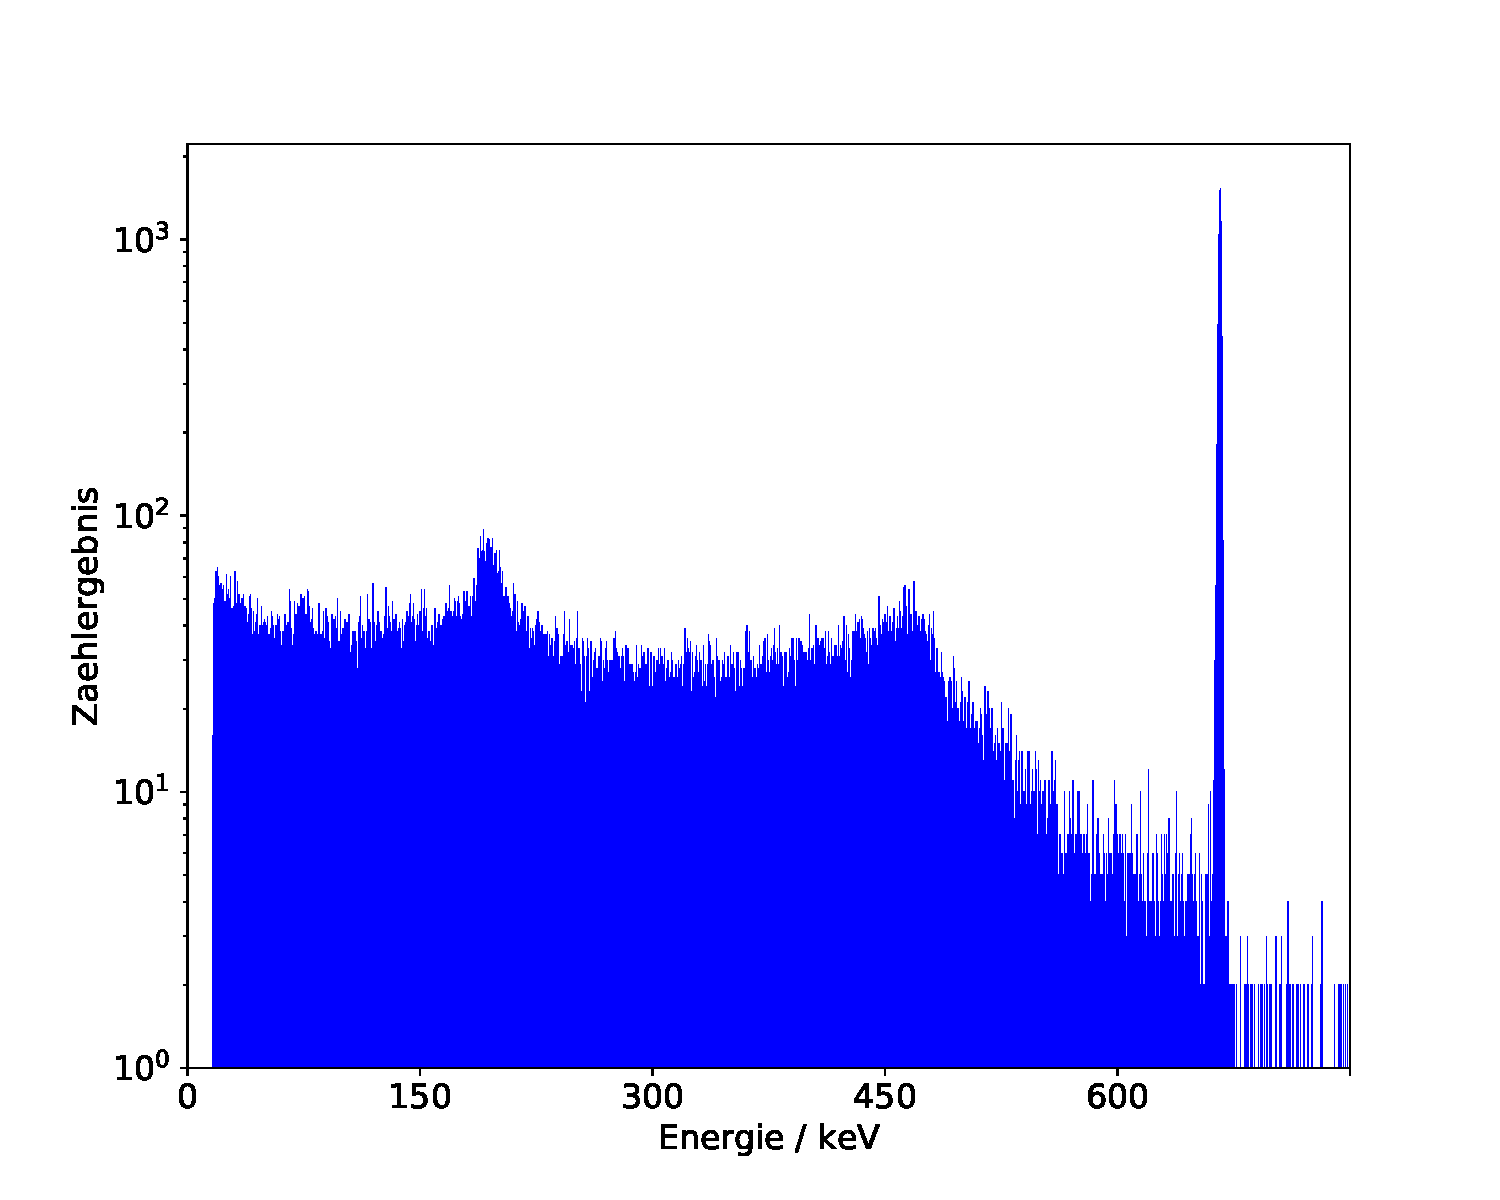
\includegraphics[width=0.8\textwidth]{python/plots/spec2.pdf}
  \caption{Spektrum des Caesium-137-Strahlers.}
  \label{fig:spectrum_caesium}
\end{figure}

\begin{figure}
  \includegraphics[width=\textwidth]{python/plots/kontinuumfit}
  \caption{Fit zur Bestimmung des Inhalts des Compton-Kontinuums.}
  \label{fig:kontinuumplot}
\end{figure}

\FloatBarrier
\subsection{Aktivitätsbestimmung von Barium 133}
\label{subsec:a3}
In Abbildung \ref{fig:Spektrum_Barium} ist das Spektrum einer Barium 133 Probe dargestellt.
\begin{figure}
\centering
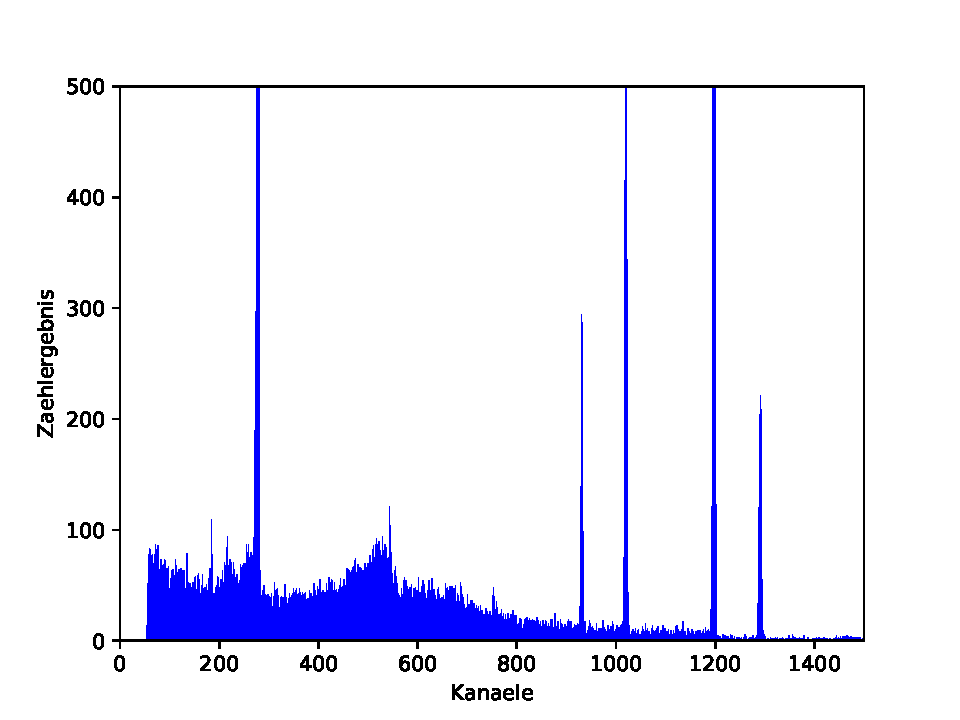
\includegraphics[width=0.8\textwidth]{python/plots/spec3.pdf}
\caption{Gamma-Spektrum einer Barium-133 Probe.}
\label{fig:Spektrum_Barium}
\end{figure}
Um die Aktivität der Probe zum Zeitpunkt der Messung zu bestimmen wird Gleichung (\ref{eqn:effizienz}) verwendet.
Wie in Abschnitt \ref{subsec:a0} beschrieben wird die Lage und der Inhalt der verschiedenen Peaks berechnet.
Mit der in Abschnitt \ref{subsec:a1} bestimmten Beziehung $Q(E)$ zwischen Effizienz und Energie, dem bekannten Raumwinkel $\Omega$ und den in Tabelle \ref{tab:a_d_1} angegebenen Emissionswahrscheinlichkeiten wird von jeder Spektrallinie einzeln auf die Aktivität der Probe geschlossen.
Die Ergebnisse dieser Rechnung finden sich ebenfalls in Tabelle \ref{tab:a_d_1}.
\begin{table}
\centering
\caption{Für die Berechnung der Aktivität wichtige Daten je Spektrallinie \cite{sample}.}
\begin{tabular}{c c c c}
\hline \\
$E_{\gamma}$ / keV & Inhalte & $W$ / \%& Aktivität / $\SI{}{\becquerel}$\\
\hline \\
53,49 $\pm$0,05  &  163  $\pm$30 &  2,20  &  90  $\pm$75 \\ 81,40 $\pm$0,01  &  8643  $\pm$217 &  34,06  &  490  $\pm$412 \\ 160,73 $\pm$0,10  &  207  $\pm$73 &  0,65  &  1310  $\pm$1253 \\ 223,29 $\pm$0,04  &  82  $\pm$14 &  0,45  &  1085  $\pm$1010 \\ 276,63 $\pm$0,01  &  1288  $\pm$22 &  7,20  &  1345  $\pm$1250 \\ 303,26 $\pm$0,01  &  3021  $\pm$59 &  18,30  &  1374  $\pm$1288 \\ 356,24 $\pm$0,00  &  8589  $\pm$80 &  62,10  &  1377  $\pm$1308 \\ 384,09 $\pm$0,02  &  1171  $\pm$38 &  8,90  &  1424  $\pm$1362 \\
\hline
\end{tabular}
\label{tab:a_d_1}
\end{table}
Als Mittelwert dieser einzelnen Aktivitäten ergibt sich das gesamt Ergebnis der Aktivität
\begin{align*}
A_{Ba-133}=\SI{1100+-500}{\becquerel} \text{ .}
\end{align*}
Die Aktivitäten, welche aus den ersten beiden Spektrallinien berechnet werden, werden bei dieser Rechnung vernachlässigt.

\FloatBarrier
\subsection{Untersuchung von Zerfallsketten in einem unbekannten Strahler }
\label{subsec:a4}
Es wird eine radioaktive Probe untersucht, deren Spektrum in Abbildung \ref{fig:spectrum_4} zu sehen ist. Die Messzeit beträgt $\SI{5016}{\second}$.
Zu untersuchen ist, welche radioaktiven Nuklide enthalten sind. Dazu werden die identifizierbaren Spektrallinien
mit denen der in der Versuchsanleitung \cite{sample} angegebenen Zerfallsreihen verglichen.  Die Position
der Spektrallinien werden, wie schon in den vorausgegangenen Abschnitten \ref{subsec:a1} und \ref{subsec:a2}, zunächst
grob aus dem aufgenommenen Spektrum abgelesen und dann genauer mithilfe eines Gauss-Fits lokalisiert.
Es ergeben sich die in Tabelle \ref{tab:spektrallinien_4}  angegebenen Spektrallinien. Es lässt sich erkennen, dass
Bestandteile der Uran-238 Zerfallsreihe auftreten. Dabei lässt sich das Glied das beginnend bei Thorium-234 (über Protactinium-234, Radium-226,
Blei-214) und endend bei Bismuth-214, gut identifizieren. Die jeweils nicht gefundenen Linien der genannten Nuklide
treten meist mit einer niedrigen Wahrscheinlichkeit auf und oder liegen bei sehr kleinen Energien. Eine Ausnahme bildet
Protactinium-234, denn hier treffen nicht immer die zuvor genannten Argumente zu. Allerdings lässt sich in diesem Fall anführen,
dass gemäß der Versuchsanleitung \cite{sample} ein zweiter Beta-zerfall mit einer Halbwertszeit von $\SI{1,2}{\minute}$ existiert. Für diesen Zerfall sind keine Spektrallinie angegeben, sodass dieser nicht detektiert werden kann.\\
In Tabelle \ref{tab:nuklide} sind die Spekrallinien der jeweiligen Nuklide aufgelistet.

\FloatBarrier
\begin{table}
  \centering
  \caption{Tabelle der in Spektrum 4 gefundenen Spektrallinien.}
  \label{tab:spektrallinien_4}
  \begin{tabular}{c c}
    \toprule
    $E \text{ in } \si{\kilo\electronvolt}$ & $ \text{zugeordnetes Nuklid} $\\
    \midrule
    \SI{1764.00+-0.00} & Bi 214 \\
    \SI{1407.62+-0.11} & Bi 214 \\
    \SI{1377.30+-0.08} & Bi 214\\
    \SI{1280.65+-0.13} &  \\
    \SI{1237.84+-0.06} & \\
    \SI{1119.97+-0.04} & Bi 214\\
    \SI{1000.85+-0.24} &  \\
    \SI{933.71+-0.07} & Bi 214 \\
    \SI{838.76+-0.14} & \\
    \SI{806.02+-0.17} &  \\
    \SI{785.76+-0.10} & Bi 212\\
    \SI{768.12+-0.04} & Bi 214 \\
    \SI{665.34+-0.06} &  \\
    \SI{609.17+-0.01} & Bi 214 \\
    \SI{351.95+-0.00} & Pb 214 \\
    \SI{295.33+-0.00} & Pb 214 \\
    \SI{242.10+-0.01} & Pb 214\\
    \SI{186.16+-0.01} & Ra 226\\
    \SI{98.34+-0.53} & Pa 234 \\
    \SI{92.95+-0.19} & Th 234\\
    \SI{77.25+-0.01} & \\
    \bottomrule
  \end{tabular}
\end{table}

\begin{table}
  \centering
  \caption{Spektrallinien der identifizierten Nuklide(Informationen aus Versuchsanleitung).\cite{sample}}
  \label{tab:nuklide}
  \begin{tabular}{c c c c c}
    \toprule
    $\text{\text{Nuklid}}$ & $E \text{ in } \si{\kilo\electronvolt}$ & $ \text{Wahrscheinlichkeit} $ & $\text{identifiziert (j/n)}$ & $\text{Begründung für Nichtidentifikation}$\\
    \midrule
    Th 234 & \SI{63}{} & \SI{3.5}{\percent} & \text{n} & \text{Energie zu gering} \\
           & \SI{93}{} & \SI{4}{\percent} & \text{j} & \\
    Pa 234 & \SI{100}{} & \SI{50}{\percent} & \text{j} & \\
           & \SI{126}{} & \SI{26}{\percent} & \text{n} & \text{alternativer beta-zerfall}\\
           & \SI{220}{} & \SI{14}{\percent} & \text{n} & \text{alternativer beta-zerfall}\\
           & \SI{360}{} & \SI{13}{\percent} & \text{n} & \text{alternativer beta-zerfall}\\
           & \SI{560}{} & \SI{15}{\percent} & \text{n} & \text{alternativer beta-zerfall}\\
           & \SI{700}{} & \SI{24}{\percent} & \text{n} & \text{alternativer beta-zerfall}\\
           & \SI{900}{} & \SI{70}{\percent} & \text{n} & \text{alternativer beta-zerfall}\\
           & \SI{1080}{} & \SI{12}{\percent} & \text{n} &  \text{alternativer beta-zerfall}\\
    Ra 226 & \SI{186}{} & \SI{4}{\percent} & \text{j} & \\
    Pb 214 & \SI{53}{} & \SI{1}{\percent} & \text{n} & \text{geringe Wahrscheinlichkeit,Energie gering} \\
           & \SI{242}{} & \SI{4}{\percent} & \text{j} & \\
           & \SI{296}{} & \SI{19}{\percent} & \text{j} & \\
           & \SI{352}{} & \SI{36}{\percent} & \text{j} & \\
    Bi 214 & \SI{609}{} & \SI{47}{\percent} & \text{j} & \\
           & \SI{769}{} & \SI{5}{\percent} & \text{j} & \\
           & \SI{935}{} & \SI{3}{\percent} & \text{j} & \\
           & \SI{1120}{} & \SI{17}{\percent} & \text{j} & \\
           & \SI{1378}{} & \SI{5}{\percent} & \text{j} & \\
           & \SI{1400}{} & \SI{4}{\percent} & \text{j} & \\
           & \SI{1509}{} & \SI{2}{\percent} & \text{n} & \text{geringe Wahrscheinlichkeit} \\
           & \SI{1728}{} & \SI{3}{\percent} & \text{n} & \text{geringe Warhscheinlichkeit} \\
           & \SI{1764}{} & \SI{17}{\percent} & \text{j} & \\
           & \SI{2204}{} & \SI{5}{\percent} & \text{n} & \text{geringe Wahrscheinlichkeit}\\
     \bottomrule
  \end{tabular}
\end{table}
\FloatBarrier

\begin{figure}
  \centering
  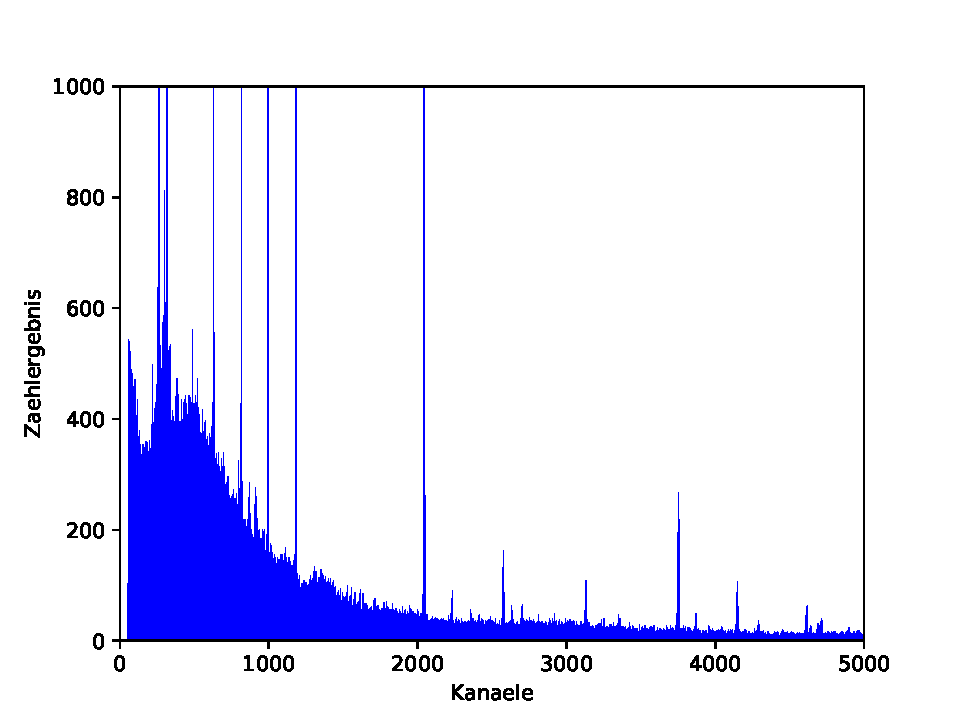
\includegraphics[width=0.8\textwidth]{python/plots/spec4}
  \caption{Spektrum des Unbekannten Strahlers.}
  \label{fig:spectrum_4}
\end{figure}



%\begin{figure}
%  \centering
%  \includegraphics{plot.pdf}
%  \caption{Plot.}
%  \label{fig:plot}
%\end{figure}
\FloatBarrier
